\chapter{Experimental Evaluation}
As mentioned in previously, this is the chapter dedicated to an experimental evaluation of the proposed framework. Firstly, there is an explanation of how the experiments are made and structured, then there is a detailed description of the DCASE dataset, already mentioned in Chapter 2, on which the proposed framework is evaluated. Successively, the chapter shows how data are prepared in order to obtain a proper output from the architecture, with a spotlight on chosen parameters.\\
In conclusion, performance metrics are described and experimental results are reported.
\section{Experimental protocol}
The experimental part of this thesis shows two instances of the proposed framework changing the way autoencoder is built and using the DCASE dataset for evaluation. In particular, two different autoencoders are taken in consideration: LSTM encoder-decoder architecture and convolutional autoencoder. The purpose of this part is in fact to show the ID conditioning effects as autoencoder layers varies, to demonstrate its compatibility with different encoding and decoding processes. Using the nature of its autoencoder, the overall architectures are so identified as ID Conditioned LSTM Autoencoder (IDC-LSTM-AE) and ID Conditioned Convolutional Autoencoder (IDCCAE). These two architectures are implemented and trained on four machines present in DCASE dataset (details reported in following sections). IDC-LSTM-AE and IDCCAE can be regarded as two possible instances of the proposed architecture.
\section{Dataset and recording procedure}
Previously, in Chapter 2, a brief introduction of DCASE 2020 TASK 2 has been done to introduce some approaches found in literature about the anomaly detection. During the experiments, a part of this dataset is used, in particular the one belonging to MIMII dataset \cite{20MIMIIDataset}.
This dataset contains audio clips recorded from four different machines: a pump, a valve, a slide rail and a fan (Table \ref{machine-descriptions}). Clips are recorded by a circular microphone array so that single-channel-based or multi-channel-based approaches can be evaluated.
\begin{figure}[ht]
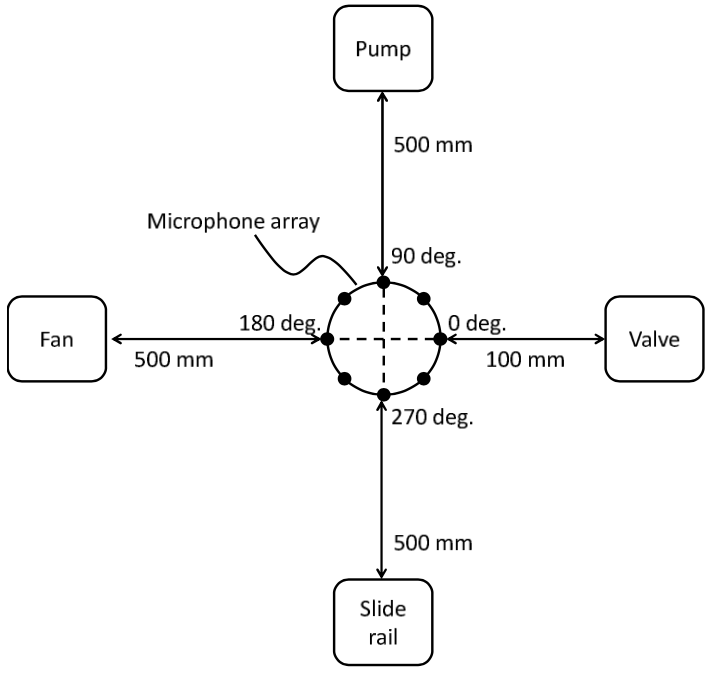
\includegraphics[scale=0.65]{TESI DI FIORE/img/micarray.png}
\centering
\caption{Microphones array disposed near machines \cite{DCASE}}
\label{micarray}
\end{figure}
Figure \ref{micarray} depicts the recording setup with the direction and distance from each machine type (each machine sound was recorded in separate sessions). To simplify the task, DCASE authors used only the first channel of multi-channel recordings and the sampling rate of all signals has been downsampled to 16 kHz. Last important thing to be noticed is the presence of real factory environmental background noise mixed with the target machine sound.\\
\begin{table}
\small
\centering
\begin{tabularx}{\textwidth}{|c|c|c|} 
\hline
\textbf{Machine Type} & \textbf{Operations} & \textbf{Some Anomalous Conditions} \\ 
\hline
Pump & \begin{tabular}[c]{@{}c@{}}Suction from/ \\discharge to a water pool\end{tabular} & \begin{tabular}[c]{@{}c@{}}Leakage, contamination, \\clogging, etc.\end{tabular} \\ 
\hline
Fan & \begin{tabular}[c]{@{}c@{}}It works to~provide a \\continuous flow or gas \\of air in factories\end{tabular} & \begin{tabular}[c]{@{}c@{}}Unbalanced, voltage change, \\clogging, etc.\end{tabular} \\ 
\hline
Slide rail & \begin{tabular}[c]{@{}c@{}}Slide repeat at \\different speeds\end{tabular} & \begin{tabular}[c]{@{}c@{}}Rail damage, loose belt, \\no grease, etc.\end{tabular} \\ 
\hline
Valve & \begin{tabular}[c]{@{}c@{}}Open/close repeat with\\~different timing\end{tabular} & \begin{tabular}[c]{@{}c@{}}More than two \\kinds of contamination\end{tabular} \\
\hline
\end{tabularx}
\caption{Machine descriptions with some anomalous conditions.}
\label{machine-descriptions}
\end{table}
DCASE 2020 authors take this dataset and arrange it in order to create \textit{development}, \textit{additional training} and \textit{evaluation} datasets. The first one contains all the necessary for autoencoder training, such as a training set and a test set, while the last one contains test data without condition labels, used for competition participants submissions. The development dataset is used for experiments. Table \ref{training-test-sets-structure} reports the machines and the number of audio clips for each of them respectively found in training and test sets.
\begin{table}[ht]
\centering
\begin{tabular}{|c|c|c|c|c|c|c|c|c|} 
\cline{2-9}
\multicolumn{1}{c|}{} & \multicolumn{2}{c|}{\textbf{ID00}} & \multicolumn{2}{c|}{\textbf{ID02}} & \multicolumn{2}{c|}{\textbf{ID04}} & \multicolumn{2}{c|}{\textbf{ID06}} \\ 
\hline
\textbf{Machine Type} & train & test & train & test & train & test & train & test \\ 
\hline
PUMP & 906 & 243 & 905 & 211 & 602 & 200 & 936 & 202 \\ 
\hline
FAN & 911 & 507 & 916 & 549 & 933 & 448 & 915 & 461 \\ 
\hline
SLIDER & 968 & 456 & 968 & 367 & 434 & 278 & 434 & 189 \\ 
\hline
VALVE & 891 & 219 & 608 & 220 & 900 & 220 & 892 & 220 \\
\hline
\end{tabular}
\caption{Training and test set structures.}
\label{training-test-sets-structure}
\end{table}
\section{Pre-Processing Phase}
In Chapter 3, mel-spectrogram extractor and all pre-processing blocks have been well described. The goal of this section is to show their details from the experimental point of view. In particular, settings and decisions made for mel-spectrogram extraction, normalization, frame generation and IDs pre-processing are presented. Regarding mel-spectrogram extraction, the same parameters are used for all machines: the number of bins ($n\_mels$) is 128, the STFT window ($n\_fft$) is 1024 and the $hop\_length$ is 512. Using Librosa functions \textit{load} and \textit{melspectrogram}, each audio clip is firstly converted into a Numpy ndarray representing the signal, successively it is converted to a mel-spectrogram and then the results are added to a final structure. The final structure contains all the extracted mel-spectrograms needed for training. Because of the duration of each clip (10 seconds) and the just mentioned parameters, each mel-spectrogram has the dimension of 128x313. Frame generation specs are reported in Table \ref{frame-generation}.\\
\begin{table}[ht]
\centering
\begin{tabular}{|c|c|c|c|c|} 
\cline{2-5}
\multicolumn{1}{c|}{} & \multicolumn{2}{c|}{\textbf{IDCCAE}} & \multicolumn{2}{c|}{\textbf{LSTM AE}} \\ 
\hline
\textbf{Machine} & \textbf{Num. Frames} & \textbf{Hop-Size} & \textbf{Num. Frames} & \textbf{Hop-Size} \\ 
\hline
Pump &  &  &  &  \\ 
\hline
Fan &  &  &  &  \\ 
\hline
Valve &  &  &  &  \\ 
\hline
Slider &  &  &  &  \\
\hline
\end{tabular}
\caption{Frame generation details.}
\label{frame-generation}
\end{table}
In particular, the column \textit{Num. Frames} report, for each machine, the number of frames extracted from each spectrogram, while \textit{Hop-Size} indicates the segmentation window shift to extract them. Regarding the normalization, a Z-Score is applied on spectrograms belonging to the same kind of machine type. For both instances of the framework, frames placed in input to autoencoders for training have the size of 128x32. In conclusion, regarding the IDs Pre-processing, the ID strings used to identify each machine kinds are $00$, $02$, $04$ and $06$ (four is the number of different kinds for each machine type) and they are converted respectively to $[0,0,0,1]$, $[0,0,1,0]$, $[0,1,0,0]$ and $[1,0,0,0]$. Moreover, for \textit{match} and \textit{not-match} transformations an $\alpha=0.75$ is chosen.

\section{Autoencoder Structure}
In this section, the structures of IDCCAE and IDC-LSTM-AE are described. In both instances, the conditioning is a sequence of mathematical operations in which encoder output and ID conditioning network outputs are involved.

\begin{figure}[ht]
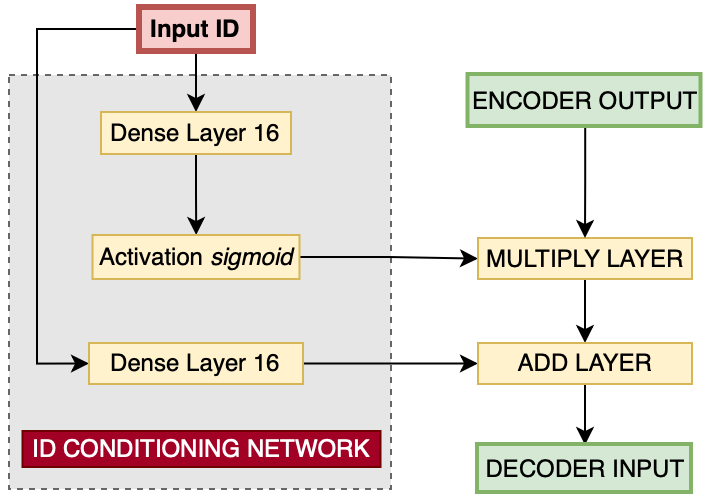
\includegraphics[scale=0.8]{TESI DI FIORE/img/CONDITIONING.png}
\centering
\caption{Conditioning operations}
\label{conditioning}
\end{figure}

The encoded ID is passed through a dense layer and an activation layer to produce the ID conditioning network first output, which is multiplied with encoder output. The second output is the output of another dense layer with the same encoded ID provided in input. To produce the final representation, which is decoder input, the second output is added to the result of the multiplication (Figure \ref{conditioning}).


\subsection{IDCCAE}

\begin{figure}[ht]
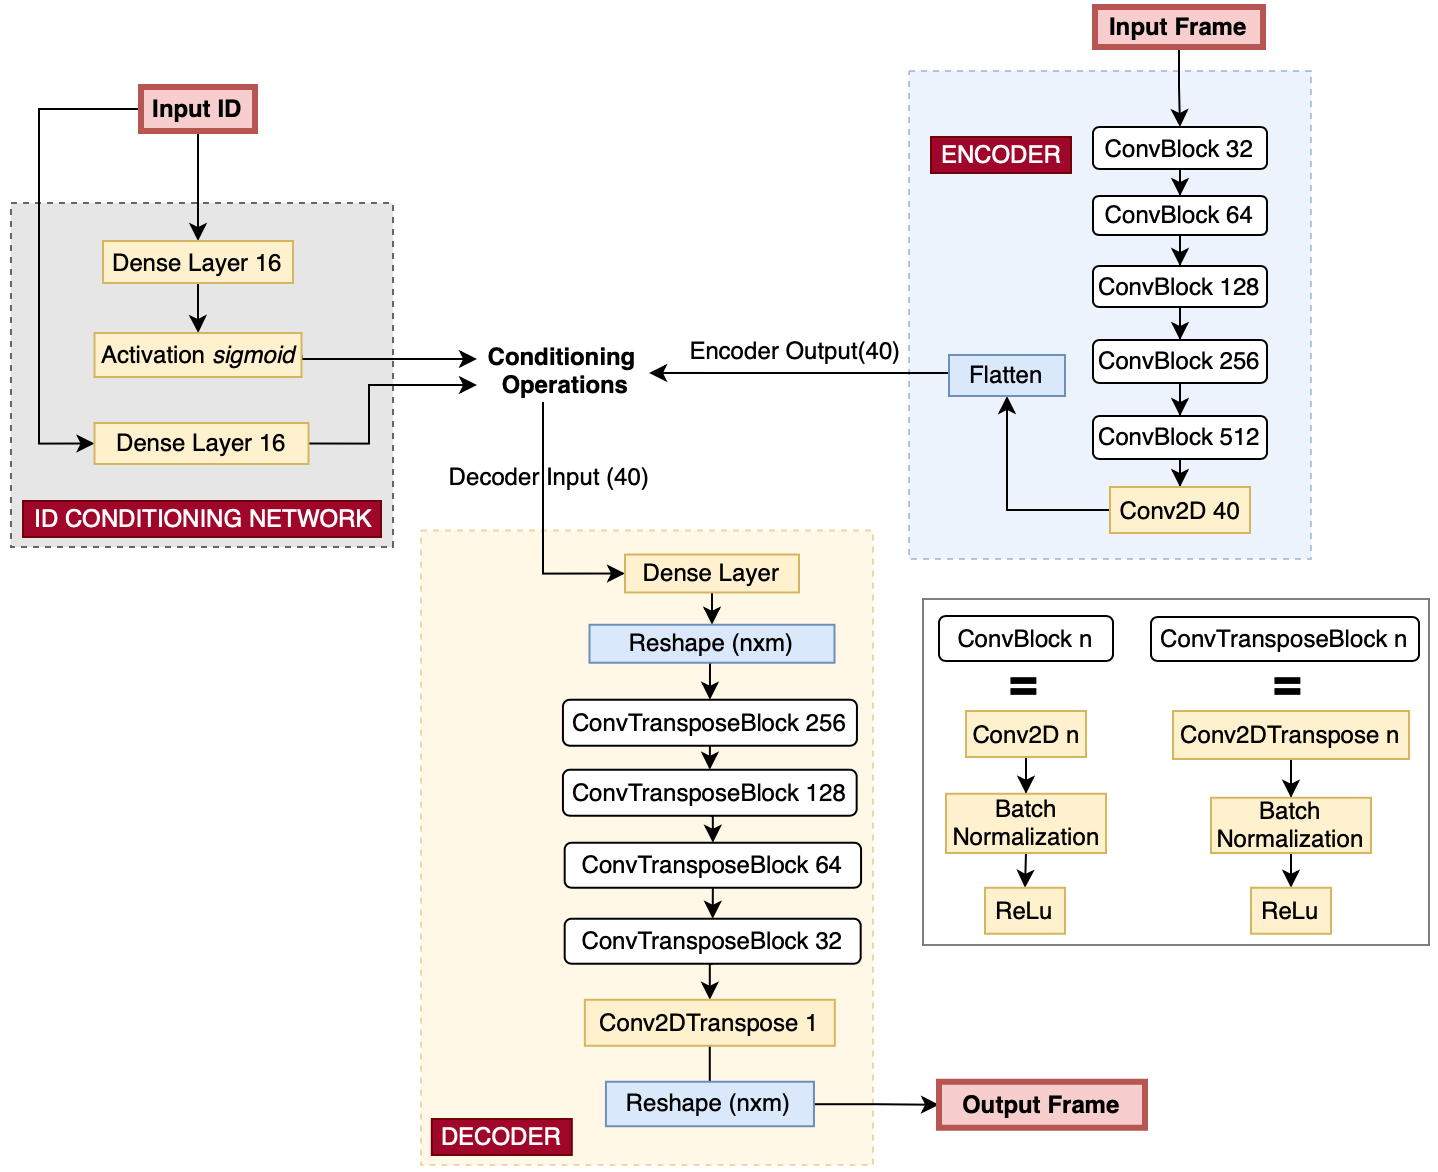
\includegraphics[scale=0.55]{TESI DI FIORE/img/IDCCAE.png}
\centering
\caption{ID Conditioned Convolutional Autoencoder}
\label{IDCCAE}
\end{figure}

The Figure \ref{IDCCAE} reports a detailed view of how encoder and decoder block are composed in the convolutional instance of the framework. The encoder network consists in a stack of five hidden layers with convolutional filters of 32, 64, 128, 256, and 512. In particular, as can be seen at the right part of the image, each component of the encoder is composed by a stack of different layers: a convolutional layer, followed by batch normalization and the ReLU activation function.\\
The bottleneck consists of a layer with 40 convolutional filters, reducing the encoder feature maps to a 40-dimensional encoded representation of the input. Regarding the decoder network, first a fully-connected layer reshapes its input to the shape of the last layer of the encoder and then five ConvTransposeBlock (Conv2DTranspose layers followed by batch normalization layers and ReLu activation functions) mirrors the encoder.\\
The conditioning operations are those explained in previous sections.

\subsection{IDC-LSTM-AE}
\begin{figure}[ht]
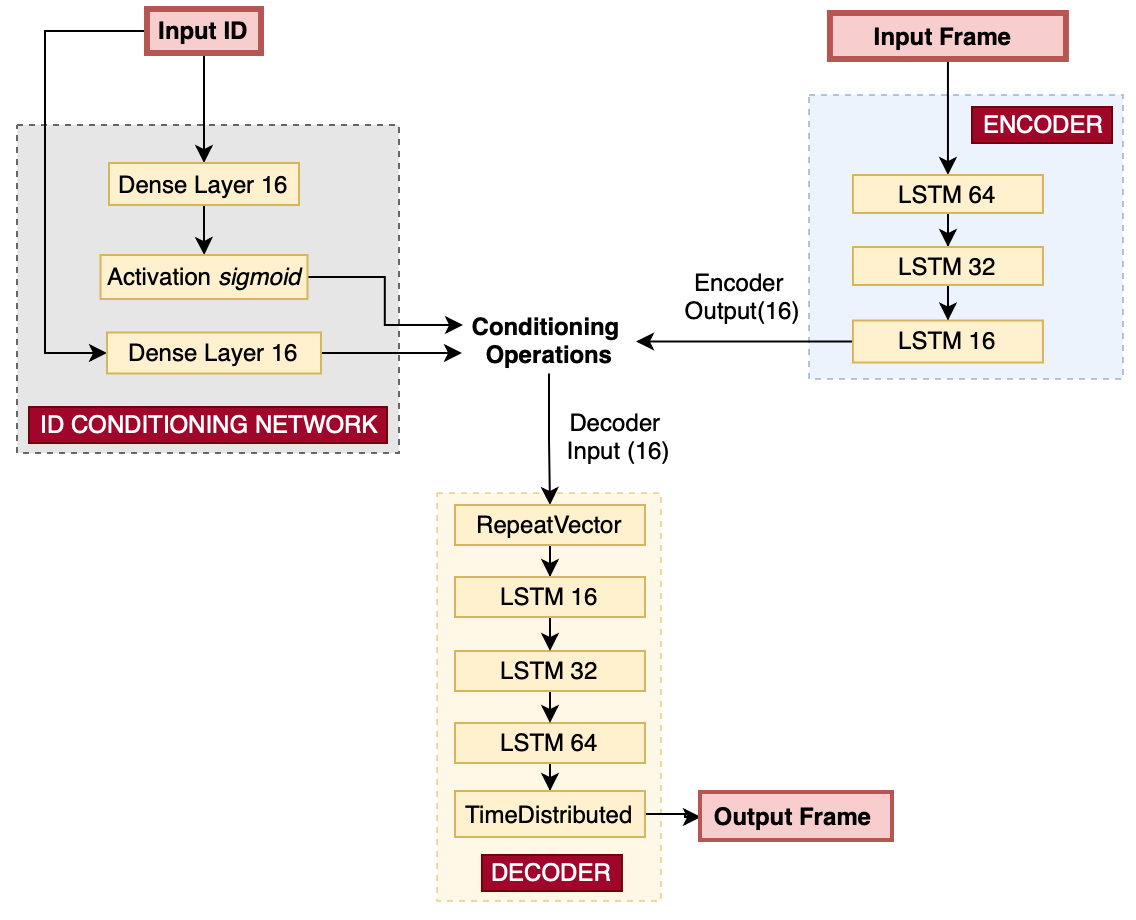
\includegraphics[scale=0.65]{TESI DI FIORE/img/LSTM-AE.png}
\centering
\caption{ID Conditioned LSTM Autoencoder}
\label{LSTM-AE}
\end{figure}
The Figure \ref{LSTM-AE} describes the architecture of the Long-Short Term Memory version of the autoencoder. Here, encoder is composed by three LSTM layers with a decreasing number of units (64,32 and 16) (which indicate the dimensionality of the output space). The decoder is the reversed version of the encoder. In this architecture, the 128x32 frames that are placed in input are seen as time-series of 32 timesteps, each of them characterized by 128 features, which are the frequency amplitudes (the $n\_mels$ bins). This architecture tries to capture the temporal relationship between sequential frequency amplitudes through time, in order to learn a function which better reconstruct the inputs.

\section{Other Hyperparameters}
In previous sections, autoencoders used to build the two instances of the proposed framework have been visualized, with an explanation of how layers are built. Obviously, during the training phase other parameters are involved, which should be optimized to get as high as possible performances. In the experimental phase of the study, in addition to those seen for IDCCAE and IDC-LSTM-AE, batch size, number of epochs and learning rate are autoencoder-independent hyperparameters taken in consideration during the tuning process. Regarding batch-size, the values $\{64,128,256,512\}$ have been attempted, while for learning rate choice, values like $\{10^{-2}, 10^{-3}, 10^{-4}, 10^{-5}\}$ are used. Number of epochs has been varied between 50 and 200.\\
The Table \ref{hyperparam-tables} reports, for the experiments made, the best hyperparameters found.

\begin{table}[ht]
\centering
\begin{tabular}{|c|c|c|c|c|c|c|} 
\cline{2-7}
\multicolumn{1}{c|}{} & \multicolumn{3}{c|}{\textbf{IDCCAE}} & \multicolumn{3}{c|}{\textbf{LSTM}} \\
\hline
\textbf{Machine} & \textbf{BS} & \textbf{EP} & \textbf{LR} & \textbf{BS} & \textbf{EP} & \textbf{LR} \\ 
\hline
Pump &  &  &  &  &  &  \\ 
\hline
Fan &  &  &  &  &  &  \\ 
\hline
Valve &  &  &  &  &  &  \\ 
\hline
Slider &  &  &  &  &  &  \\
\hline
\end{tabular}
\caption{Batch size (BS), learning rate (LR) and number of epochs (EP) chosen. These parameters are used to get final results of the experimental part of this text.}
\label{hyperparam-tables}
\end{table}

\section{Evaluation and Performance Metrics}
The goal of this section is to explain how the performances of trained models are evaluated. First of all, in both cases the test sets are pre-processed in the same way seen for training sets. Regarding the metrics used for models evaluation during the experiments, the area under the receiver operating characteristic (ROC) curve (AUC) and the partial-AUC (pAUC) are considered. These metrics are the same metrics used for the competition ranking, when the challenge was still in progress. Remembering that the ROC curve shows the trend of the true positive rate (TPR) in function of the false positive rate (FPR) at the variation of a parameter (like the threshold used for binary classification tasks), the pAUC is calculated as the AUC over a low FPR range $[0,p]$. Following, there are the formulas reported by \cite{DCASE}:
\[ AUC =\frac{1}{N_-N_+}\sum_{i=1}^{N_-}\sum_{j=1}^{N_+}\mathcal{H}(A_\theta(x_j^+)-A_\theta(x_i^-)) \]
\[AUC =\frac{1}{ \left \lfloor pN_- \right \rfloor N_+}\sum_{i=1}^{ \left \lfloor pN_- \right \rfloor }\sum_{j=1}^{N_+}\mathcal{H}(A_\theta(x_j^+)-A_\theta(x_i^-))\]
where $A_\theta(\cdot)$ is the anomaly score generated by the autoencoder, ⌊⋅⌋ is the flooring function and $\mathcal{H}$ returns 1 when $x>0$ and $0$ otherwise. Here, $\{x^−_i\}^{N_-}_{i=1}$
and $\{x^+_j\}^{N_+}_{j=1}$ are normal and anomalous test samples, respectively, and have been sorted so that their anomaly scores are in descending order. Here, $N_−$ and $N_+$
are the number of normal and anomalous test samples, respectively. According to the above formulas, the anomaly scores of normal test samples are used as the threshold. If an ASD system gives false alerts frequently, we cannot trust it. For these reasons, it is especially important to increase the TPR under low FPR conditions. In this task, we will use $p=0.1$. In conclusion, because the results produced with a GPU are generally non-deterministic, the averages and standard deviations are calculated from 10 independent trials (training and testing). The next section reports results tables.

\section{Results}
This section compares the results obtained from the training of the two models just described and the results published by DCASE authors. The IDCCAE architecture is compared with a similar version of the architecture without the ID conditioning mechanism \cite{15DeepDenseConvAE}. The IDC-LSTM-AE, in the same way, is evaluated using the results obtained by \cite{16LSTMDeepAutoencodersForASDtask}, in which a similar LSTM autoencoder without conditioning is trained. 
Moreover, both the proposed architectures, are compared with the baseline results provided by the authors of the challenge and with the results obtained by the authors of \cite{18IDConditionedAutoEncoder}, which have trained an autoencoder with fully connected layers and with the conditioning mechanism.

\begin{table}[ht]
\centering
\begin{tabular}{|c|c|c|c|c|c|c|c|c|} 
\cline{2-9}
\multicolumn{1}{c|}{} & \multicolumn{2}{c|}{\textbf{Pump}} & \multicolumn{2}{c|}{\textbf{Fan}} & \multicolumn{2}{c|}{\textbf{Slider}} & \multicolumn{2}{c|}{\textbf{Valve}} \\ 
\hline
\textbf{Architecture} & AUC & pAUC & AUC & pAUC & AUC & pAUC & AUC & pAUC \\ 
\hline
Baseline &  &  &  &  &  &  &  &  \\ 
\hline
IDCAE &  &  &  &  &  &  &  &  \\ 
\hline
IDCCAE &  &  &  &  &  &  &  &  \\ 
\hline
LSTM &  &  &  &  &  &  &  &  \\
\hline
\end{tabular}
\caption{Average of AUC and pAUC for different architectures on 10 indipendent trials (training and testing).}
\label{datasets-average-results}
\end{table}
\begin{table}[ht]
\centering
\begin{tabular}{|c|c|c|c|c|c|c|c|c|} 
\cline{2-9}
\multicolumn{1}{c|}{} & \multicolumn{2}{c|}{\textbf{Pump}} & \multicolumn{2}{c|}{\textbf{Fan}} & \multicolumn{2}{c|}{\textbf{Slider}} & \multicolumn{2}{c|}{\textbf{Valve}} \\ 
\hline
\textbf{Architecture} & AUC & pAUC & AUC & pAUC & AUC & pAUC & AUC & pAUC \\ 
\hline
Baseline &  &  &  &  &  &  &  &  \\ 
\hline
IDCAE &  &  &  &  &  &  &  &  \\ 
\hline
IDCCAE &  &  &  &  &  &  &  &  \\ 
\hline
LSTM &  &  &  &  &  &  &  &  \\
\hline
\end{tabular}
\caption{Standard deviations of AUC and pAUC for different architectures on 10 indipendent trials (training and testing).}
\label{datasets-std-dev-results}
\end{table}

\section{Threshold Definition}
In Chapter 3, an online version of the proposed framework is shown. It allows a real-time audio classification to establish if a machine is working in a normal state or not. From a technical point of view, the online architecture uses the autoencoder, trained with the offline procedures, to reconstruct the spectrograms placed in input. After a reconstruction error evaluation, on the basis of a threshold, the audio is classified. Once obtained reconstruction errors, used as anomaly scores, AUC and pAUC are used to compare different solutions and approaches, but threshold definition step should be done to commission the anomalous sound detector, because without it models can't classify audio inputs. This section tries to explain a possible way to calculate an optimal threshold, but it is not the only one. In fact, a lot of literature and different approaches can be found on threshold calculation optimization process, but this question is beyond the scope of this text. \\
To calculate an optimal threshold, the concept of optimal must be examined. It depends on the particular use case taken in exam. In fact, once defined a threshold $\epsilon$ and a test set is evaluated, a confusion matrix could be calculated, from which true positive rate (TPR, where positive means anomalous), false positive rate (FPR) and other important measures can be extracted. The threshold goodness is related to the weights and the importance associated to this measures. In anomaly detection task is important to have high TPR and as low as possible value of FPR. To this purpose, the Youden's index J is defined\cite{13RealTimeDetectionUsingSequentialAutoencoder}:
\[ J = Sensitivity + Specificity - 1\]\[ Sensitivity = TPR = \frac{TP}{TP+FN}\]\[ Specificity = TNR = \frac{TN}{TN+FP} = 1-FPR = 1-\frac{FP}{TN+FP}\]\[ J = TPR+(1-FPR)-1 = TPR-FPR \]
The higher J is, better the threshold is, according to this definition of optimum. To achieve the best, the threshold that corresponds to the max value of J must be found.\\
Practically, the optimal threshold is calculated using following steps:
\begin{enumerate}
    \item {Collection of the reconstruction errors calculated from test set samples, which are anomaly scores.}
    \item {Using scikit-learn function \textit{metrics.roc\_curve} FPR, TPR and Thresholds, also used to visualize ROC curve are calculated. FPR, TPR and Thresholds are three arrays of the same length.}
    \item {The optimal threshold corresponds to the element of Thresholds array at the index on which there is a maximum value of $TPR-FPR$. In other way, a vector of the differences between TPR and FPR can be calculated and then the index of the maximum difference on this vector is the index of the optimal threshold in Threshold array.}
\end{enumerate}
Following, Figure \ref{roc_curves} shows the ROC curves calculated for IDCCAE architecture trained on audio clips recorded from pumps. It shows the ROC curves in blue and the bisector lines in red. Dashed lines indicates the values of J. Moreover, red dot is used to mark the FPR and TPR which correspond to the optimal threshold. The value of the latter is also reported.
\begin{figure}[ht]
\centering
\begin{subfigure}
    \centering
    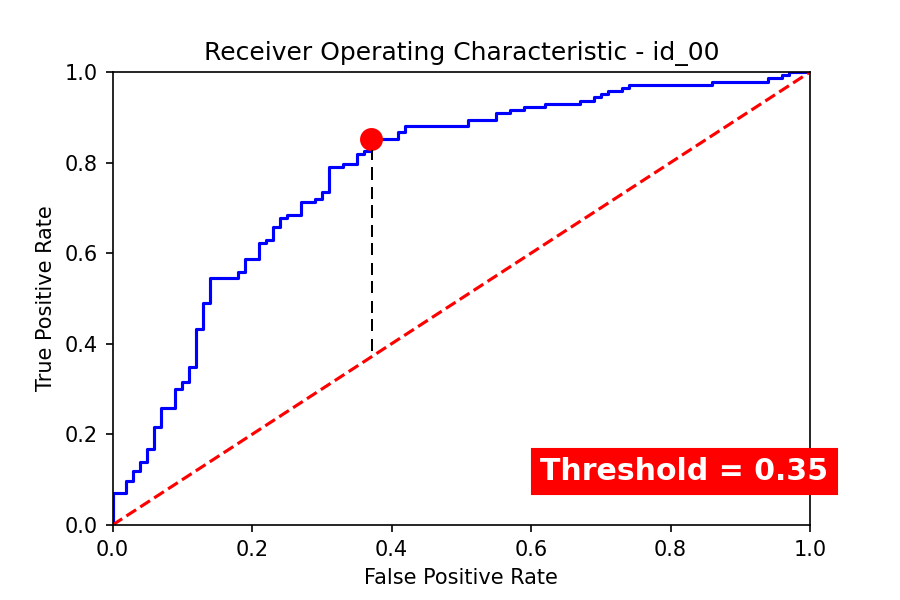
\includegraphics[scale=0.47]{TESI DI FIORE/img/roc_id_00.png}
\end{subfigure}
\begin{subfigure}
    \centering
    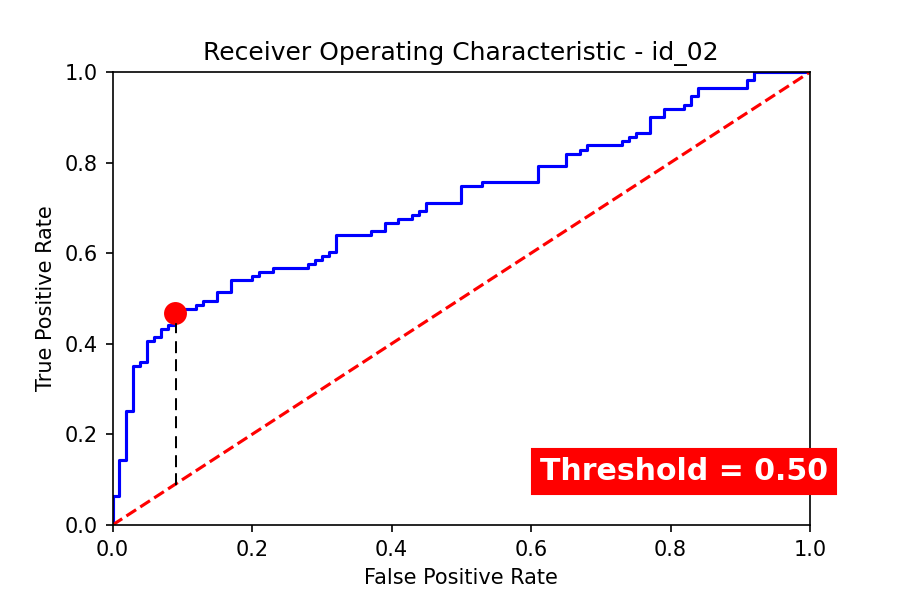
\includegraphics[scale=0.47]{TESI DI FIORE/img/roc_id_02.png}
\end{subfigure}
\begin{subfigure}
    \centering
    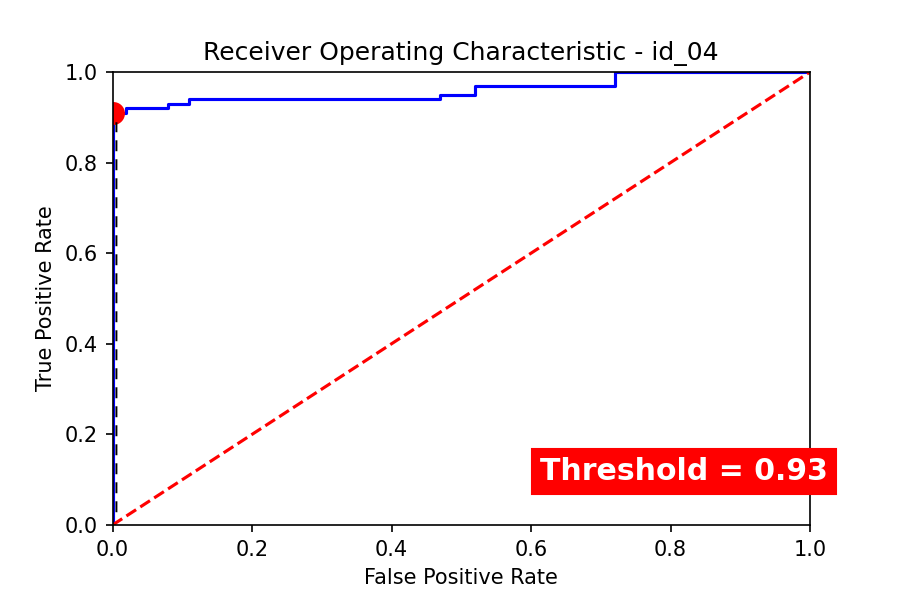
\includegraphics[scale=0.47]{TESI DI FIORE/img/roc_id_04.png}
\end{subfigure}
\begin{subfigure}
    \centering
    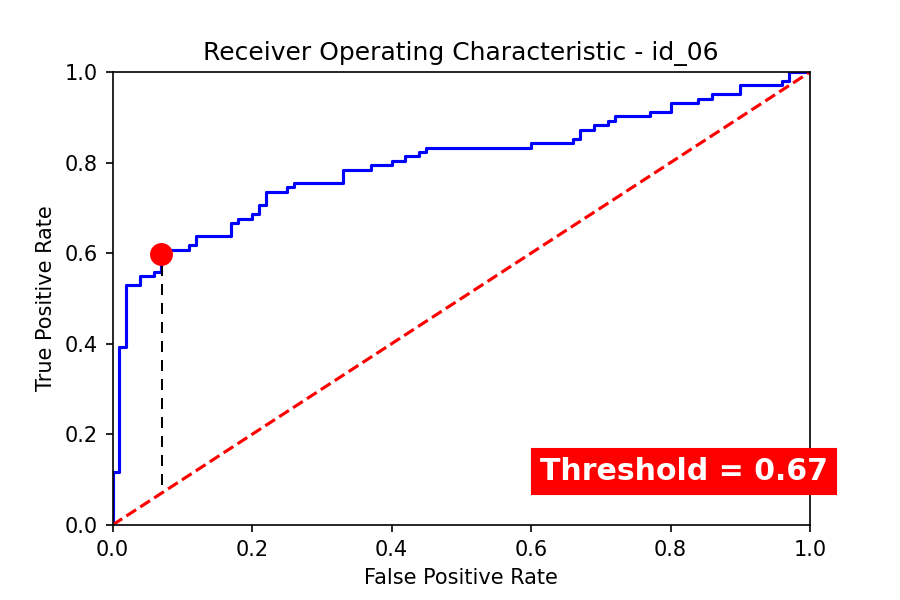
\includegraphics[scale=0.47]{TESI DI FIORE/img/roc_id_06.png}
\end{subfigure}
\begin{subfigure}
    \centering
    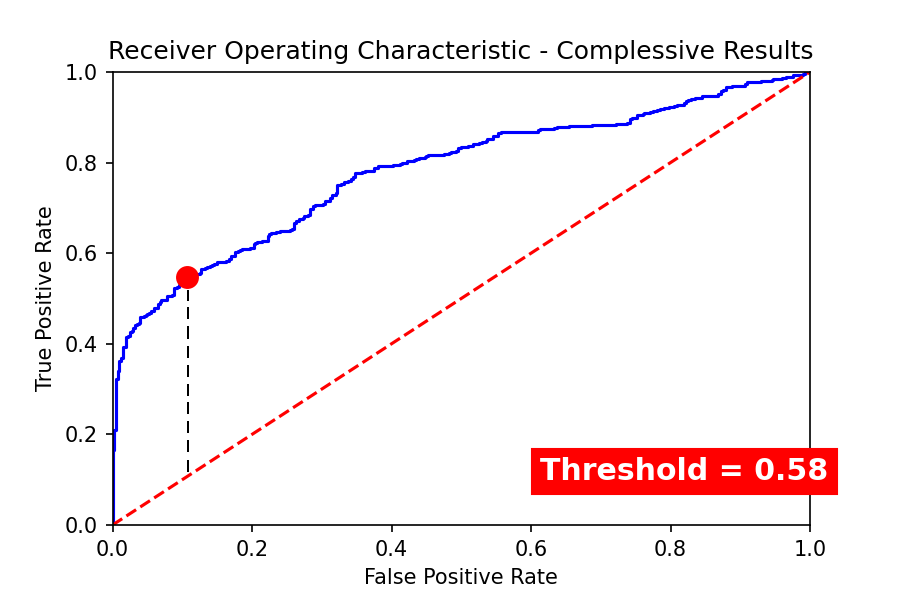
\includegraphics[scale=0.47]{TESI DI FIORE/img/roc_complessive.png}
\end{subfigure}
\caption{ ROC curves obtained using IDCCAE model on pumps test audio clips. The images shown below is the ROC curve calculated using the predictions of all four kinds of pump, with the threshold calculated.}
\label{roc_curves}
\end{figure}
In online detection phases, two alternatives should be taken in consideration:
\begin{itemize}
    \item {Use a different threshold for each ID string (or machine kind), even if the model used for prediction is one;}
    \item {Use only one threshold, regardless of the different machine kinds (last Figure \ref{roc_curves}).}
\end{itemize}
This procedure can also be applied to IDC-LSTM-AE and for all machine types.